\documentclass[beamer,crop,tikz]{standalone}

\usepackage{formation}
\usepackage{tikz}

\usetikzlibrary{matrix, positioning, arrows.meta}


\begin{document}

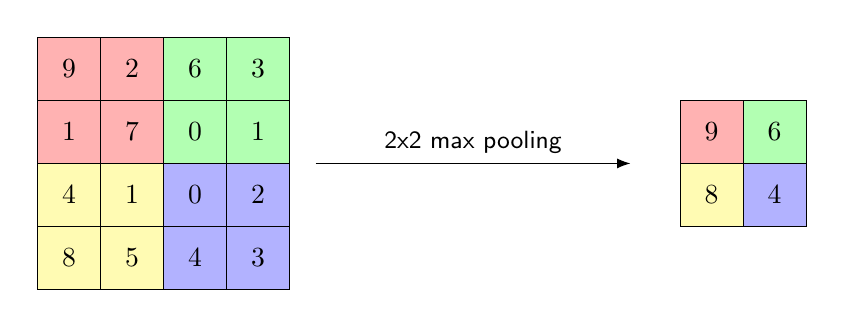
\begin{tikzpicture}

\matrix[matrix of nodes,
    column sep=-\pgflinewidth,
    row sep=-\pgflinewidth,
    nodes={anchor=center, minimum size=8mm, fill=red!30, draw}] (LeftMatrix)
{9 & 2 &|[fill=green!30]| 6 &|[fill=green!30]| 3\\
1 & 7 &|[fill=green!30]| 0 &|[fill=green!30]| 1 \\
|[fill=yellow!30]|4 &|[fill=yellow!30]| 1 &|[fill=blue!30]| 0 &|[fill=blue!30]| 2 \\
|[fill=yellow!30]|8 &|[fill=yellow!30]| 5 &|[fill=blue!30]| 4 &|[fill=blue!30]| 3 \\};
 \draw[-{LaTeX}] ([xshift=2mm]LeftMatrix.east) -- node[above, align=left, font=\sffamily\small] {2x2 max pooling} ++(0:4cm) coordinate(aux);
\matrix[matrix of nodes,
    column sep=-\pgflinewidth,
    row sep=-\pgflinewidth,
    nodes={anchor=center, minimum size=8mm, fill=red!30, draw}, right=5mm of aux] (RightMatrix)
{9 & |[fill=green!30]| 6\\
|[fill=yellow!30]| 8 & |[fill=blue!30]| 4 \\};
 
  
\end{tikzpicture}
\end{document}